%% This Beamer template is based on the one found here: https://github.com/sanhacheong/stanford-beamer-presentation, and edited to be used for Stanford ARM Lab

\documentclass[10pt, aspectratio=169]{beamer}
%\mode<presentation>{}

\usepackage{media9}
\usepackage{amssymb,amsmath,amsthm,enumerate}
\usepackage[utf8]{inputenc}
\usepackage{array}
\usepackage[parfill]{parskip}
\usepackage{graphicx}
\usepackage{caption}
\usepackage{subcaption}
\usepackage{bm}
\usepackage{amsfonts,amscd}
\usepackage[]{units}
\usepackage{listings}
\usepackage{multicol}
\usepackage{multirow}
\usepackage{tcolorbox}
\usepackage{physics}
\usepackage{algpseudocode}
\usepackage{mathtools}
\usepackage{algorithmicx, algorithm2e}
% \usepackage{xcolor}

% Enable colored hyperlinks
\hypersetup{
    colorlinks=true,
    citecolor=uma_pink,
    linkcolor=uma_blue_light,
    filecolor=uma_blue_water,      
    urlcolor=uma_blue_light,
    pdftitle={Overleaf Example},
    pdfpagemode=FullScreen,
}

% Select normal math font
\usefonttheme[onlymath]{serif}

\renewcommand{\thebibliography}{\textcolor{uma_blue_water}{\arabic{bibliography}}}
\renewcommand{\thefigure}{\textcolor{uma_blue_water}{\arabic{figure}}}
\renewcommand{\figurename}{\textcolor{uma_blue_water}{Fig.}}
\renewcommand{\thesubfigure}{\textcolor{uma_blue_water}{\alph{subfigure}}}
\renewcommand{\thetable}{\textcolor{uma_blue_water}{\arabic{table}}}
\renewcommand{\tablename}{\textcolor{uma_blue_water}{Table}}


% The following three lines are for crossmarks & checkmarks
\usepackage{pifont}% http://ctan.org/pkg/pifont
\newcommand{\cmark}{\ding{51}}%
\newcommand{\xmark}{\ding{55}}%

% Numbered captions of tables, pictures, etc.
\setbeamertemplate{caption}[numbered]

%\usepackage[superscript,biblabel]{cite}
\usepackage{algorithm2e}
\renewcommand{\thealgocf}{}

% Bibliography settings
\usepackage[style=ieee]{biblatex}
\setbeamertemplate{bibliography item}{\insertbiblabel}
\addbibresource{references.bib}

% Glossary entries
\usepackage[acronym]{glossaries}
\newacronym{ML}{ML}{machine learning}
\newacronym{HRI}{HRI}{human-robot interactions}
\newacronym{RNN}{RNN}{Recurrent Neural Network}
\newacronym{LSTM}{LSTM}{Long Short-Term Memory}


\theoremstyle{remark}
\newtheorem*{remark}{Remark}
\theoremstyle{definition}

\newcommand{\empy}[1]{{\color{uma_blue_dark}\emph{#1}}}
\newcommand{\empr}[1]{{\color{uma_blue_dark}\emph{#1}}}
\newcommand{\examplebox}[2]{
\begin{tcolorbox}[colframe=uma_blue_dark,colback=uma_gray_light,title=#1]
#2
\end{tcolorbox}}

\usetheme{Uma} 
\def \i  {\item}
\def \ai {\item[] \quad \arrowbullet}
\newcommand \si[1]{\item[] \quad \bulletcolor{#1}}
\def \wi {\item[] \quad $\ \phantom{\Rightarrow}\ $}
\def \bi {\begin{itemize}\item}
\def \ei {\end{itemize}}
\def \be {\begin{equation*}}
\def \ee {\end{equation*}}
\def \bie {$\displaystyle{}
\def \eie {{\ }$}}
\def \bsie {\small$\displaystyle{}
\def \esie {{\ }$}\normalsize\selectfont}
\def \bse {\small\begin{equation*}}
\def \ese {\end{equation*}\normalsize}
\def \bfe {\footnotesize\begin{equation*}}
\def \efe {\end{equation*}\normalsize}
\renewcommand \le[1] {\\ \medskip \lefteqn{\hspace{1cm}#1} \medskip}
\def \bex {\begin{example}}
\def \eex {\end{example}}
\def \bfig {\begin{figure}}
\def \efig {\end{figure}}
\def \btheo {\begin{theorem}}
\def \etheo {\end{theorem}}
\def \bc {\begin{columns}}
\def \ec {\end{columns}}
\def \btab {\begin{tabbing}}
\def \etab {\end{tabbing}\svneg\svneg}
\newcommand \col[1]{\column{#1\linewidth}}
\def\vneg  {\vspace{-5mm}}
\def\lvneg {\vspace{-10mm}}
\def\svneg {\vspace{-2mm}}
\def\tvneg {\vspace{-1mm}}
\def\vpos  {\vspace{5mm}}
\def\lvpos {\vspace{10mm}}
\def\svpos {\vspace{2mm}}
\def\tvpos {\vspace{1mm}}
\def\hneg  {\hspace{-5mm}}
\def\lhneg {\hspace{-10mm}}
\def\shneg {\hspace{-2mm}}
\def\thneg {\hspace{-1mm}}
\def\hpos  {\hspace{5mm}}
\def\lhpos {\hspace{10mm}}
\def\shpos {\hspace{2mm}}

\logo{
\includegraphics[height=0.8cm]{./style_files_uma/logo_uma_negativo}\hspace{0.1cm}}

% commands to relax beamer and subfig conflicts
% see here: https://tex.stackexchange.com/questions/426088/texlive-pretest-2018-beamer-and-subfig-collide
\makeatletter
\let\@@magyar@captionfix\relax
\makeatother

\title[\href{https://jmgandarias.com}{\textcolor{white}{jmgandarias.com}}]{Trajectory Planning in the Operational Space}

%\subtitle{Subtitle Of Presentation}

%\beamertemplatenavigationsymbolsempty

\begin{document}

\author[Systems Engineering and Automation]{
	\large
	Juan M. Gandarias\\
    \footnotesize \href{mailto:jmgandarias@uma.es}{jmgandarias@uma.es}
}

\institute{
	\textcolor{uma_gray_dark}{
    Systems Engineering and Automation Department\\
	University of Malaga\\
    \href{https://www.uma.es/imech/}{IMECH.UMA}}
 	\vskip 5pt
    % \small{\date{\today}}
 %    \begin{figure}
	% 	\centering
	% 	\begin{subfigure}[t]{0.5\textwidth}
	% 		\centering
	% 		
\includegraphics[height=1.5cm]{./style_files_uma/logo_uma}
	% 	\end{subfigure}%
	% 	~
	% 	\begin{subfigure}[t]{0.5\textwidth}
	% 		\centering
	% 		\includegraphics[height=0.33in]{./images/arm_lab_logo_with_title_small_adj_6.png}
	% 	\end{subfigure}
	% \end{figure}
}


\date{\today}

\begin{noheadline}
\begin{frame}
    \maketitle
    \vspace{-1cm}
    \begin{figure}
		\centering
		
\includegraphics[height=1.5cm]{./style_files_uma/logo_uma}
        \hspace{10cm}
        
\includegraphics[height=1.4cm]{./style_files_uma/logo_isa}
	\end{figure}
 %    \begin{figure}
	% 	\centering
	% 	\begin{subfigure}[t]{0.5\textwidth}
	% 		\centering
	% 		
\includegraphics[height=1.5cm]{./style_files_uma/logo_uma}
	% 	\end{subfigure}%
	% 	~
	% 	\begin{subfigure}[t]{0.5\textwidth}
	% 		\centering
	% 		\includegraphics[height=0.33in]{./images/arm_lab_logo_with_title_small_adj_6.png}
	% 	\end{subfigure}
	% \end{figure}
 \end{frame}
\end{noheadline}



\setbeamertemplate{itemize items}[circle]
% \setbeamertemplate{itemize subitem}[square]

\begin{frame}
	\frametitle{Overview} % Table of contents slide, comment this block out to remove it
	\tableofcontents % Throughout your presentation, if you choose to use \section{} and \subsection{} commands, these will automatically be printed on this slide as an overview of your presentation
\end{frame}



\section{Introduction}

\begin{frame}[allowframebreaks]
\frametitle{Introduction}
	\begin{itemize}
    
	    \item \textbf{Trajectory Planning:} To generate the references to the motion control system of a robotic manipulator.
        \begin{itemize}
            \item References are computed from a polynomial that adjusts to the desired trajectory.
            \item During the whole motion from the initial to the last pose the actuators are not saturated (smooth trajectories).
        \end{itemize}
        
    \item \textbf{Path:} Sequence of points in the joint or operational (Cartesian) space. 
    
    \item \textbf{Trajectory:} Path with a temporal law in terms of velocity or acceleration (path + schedule) \cite{paths_and_trajectories}.
    
    \item \textbf{Joint space:} Set of all possible positions and orientations of a robot's joints (a.k.a. configuration space).
    
    $\mathbf{q} = [q_1, ..., q_n ]^T \in \mathbb{R}^n$, $n \equiv \textrm{number of joint DoFs}$ 

    \framebreak
    
    \item \textbf{Operational space:} Space in which the robot's end-effector operates. Defined by the EE pose (a.k.a. task space).

    \item \textbf{Cartesian space:} Operational space described by the Cartesian coordinates and orientation angles.
    
    $\mathbf{x} = [\underbrace{x, y, z}_{position}, \underbrace{\alpha_x, \alpha_y, \alpha_z}_{orientation}] \in \mathbb{R}^6$.

    \item \textbf{Kinematics:} Study of motion without forces

    \begin{itemize}
        \item Forward kinematics: $\mathbf{x} = f(\mathbf{q})$
        \item Inverse kinematics: $\mathbf{q} = g(\mathbf{x})$
        \item First-order differential kinematics (Jacobian): $\mathbf{\dot{x}} = \mathbf{J}(\mathbf{q})\mathbf{\dot{q}}$, \hspace{0.2cm} $\mathbf{\dot{q}} = \mathbf{J}^{-1}(\mathbf{q})\mathbf{\dot{x}}$
    \end{itemize}
    
	\end{itemize}

    \framebreak

    \begin{center}
    \begin{minipage}{.45\linewidth}
    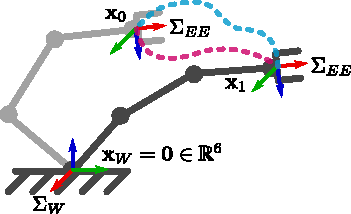
\includegraphics{images/manipulator_path.pdf}
    \end{minipage}%
    \begin{minipage}{.6\linewidth}
    \begin{itemize}
        \item $\mathbf{x}_0$ and $\mathbf{x}_1$ are EE poses w.r.t. $\mathbf{\Sigma}_W$
        \item Thanks to inverse kinematics, we can calculate $\mathbf{q}_1 = g(\mathbf{x}_1)$ 
        \item If we set this value to the motors, the robot will move towards that pose
        \item But...
        \begin{itemize}
            \item Which path will be followed?
            \item Which trajectory? 
            \item How can we control it? $\rightarrow$ Trajectory Planning
        \end{itemize}
    \end{itemize}
    \end{minipage}
    \end{center}

    \framebreak
    \begin{itemize}
        \item If there is an obstacle in the way of the robot, or if we want the robot to keep a specific orientation over the path (e.g., it carries a glass of water) $\Rightarrow$ \textcolor{uma_pink}{WE NEED A TRAJECTORY}
        \item \textbf{Generating the path:} Calculate a set of intermediate pose references (waypoints).
        \item \textbf{Generating the trajectory:} 
        \begin{enumerate}
            \item Set the arrival times to each of these waypoints.
            \item Define the polynomial to ensure a smooth trajectory.
        \end{enumerate}

        \vspace{0.5cm}
        \centering
        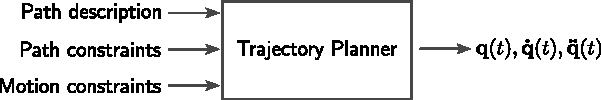
\includegraphics{images/trajectory_planner_schema.pdf}
    \end{itemize}

    \framebreak
    Two trajectory Planning approaches:
    
    \begin{center}
    \begin{minipage}[t]{.5\linewidth}
        \textbf{\textcolor{uma_blue_dark}{Trajectories in the Joint Space:}}
        \begin{itemize}
            \item Planning in terms of controlled variables $(\mathbf{q}(t))$.
            \item A polynomial is generated for each joint.
            \item Lightweight computation.
            \item Easy to compute in real-time.
            \item Hard to determine the actual Cartesian motion.
            \item The EE trajectory is not controllable.
        \end{itemize}
    \end{minipage}
    \begin{minipage}[t]{.49\linewidth}
        \textbf{\textcolor{uma_blue_dark}{Trajectories in the Operational Space:}}
        \begin{itemize}
            \item Essential for tasks in the operational space.
            \item The EE Cartesian trajectory is known.
            \item Need to compute inverse kinematics (including $\mathbf{J}^{-1}$).
            \item Higher computational cost.
            \item Have to deal with singularities.
            \item The orientation is not unique.
            
        \end{itemize}
    \end{minipage}
    \end{center}

  
\end{frame}

\section{Trajectory Planning in the Joint Space}
\begin{frame}[allowframebreaks]
\frametitle{Trajectory Planning in the Joint Space}

\textbf{\textcolor{uma_blue_dark}{Algorithm}}

\begin{minipage}[T!]{.48\linewidth}
\begin{algorithm}[H]
	$\mathbf{X} \gets \textsf{Knots}$\;
    $\mathbf{Q} = \textsf{inverse\_kinematics}(\mathbf{X})$\;
    $\mathcal{H}(t) \gets \mathcal{J}(\mathbf{Q}, t_f)$\;
    $t_k = 0$\;
	\While{$t_k < t_f$}
 	{
        $t_k = t_k + \Delta t$\;
        $\mathbf{q}_{d} = \mathcal{H}(t_k)$\;
        publish($\mathbf{q}_{d}$)\;
        sleep($\Delta t$);
  	}
\end{algorithm}
\end{minipage}
\begin{minipage}[T!]{.42\linewidth}
\begin{itemize}
    \item $\mathbf{X} = [\mathbf{x}_0, \dots, \mathbf{x}_l]\in\mathbb{R}^{6 \times l}$
    \item $\mathbf{Q} = [\mathbf{q}_0, \dots, \mathbf{q}_l]\in\mathbb{R}^{n \times l}$
    \item $\mathcal{J}\equiv$ polynomial interpolation.
    \item $l \equiv$ number of locations (knots).
    \item $t_k \equiv$ time at step $k$.
    \item $t_f \equiv$ final time.
    \item We get a trajectory for each joint (by interpolation).
    \item Not a Cartesian trajectory.
\end{itemize}
\end{minipage}

Different types of $\boldsymbol{h}(\mathbf{Q}, t_f)$ (already studied in Robot Programming and Control)~\cite{joint_trajectory_planning}:
\begin{itemize}
    \item Cubic polynomials, Quintic polynomials, Linear Segments with Parabolic Blends (LSPB)~\cite{point_to_point}.
\end{itemize}


\end{frame}

\section{Trajectory Planning in the Cartesian Space}
\begin{frame}[allowframebreaks]
\frametitle{Trajectory Planning in the Operational Space}

\begin{itemize}
    \item We must schedule the Cartesian locations (poses) of the EE between the initial and final poses~\cite{cartesian_trajectory_planning}.
    \item The polynomial interpolation is conducted in the Operational Space (Cartesian interpolation):
    
    $
    \mathbf{h}(t_k) = \textsf{cartesian\_interpolation}(\mathbf{x}, t_f)\in\mathbb{R}^6
    $
    
    \item Position and Orientation along the generated Cartesian path must be defined separately (different representations).
    \item High actuators control frequency $\rightarrow$ real-time.
    \item The number of Cartesian locations (knots) to be interpolated in the Cartesian space is typically low (2 knots for point-to-point, 2 knots if using a via point).
    \item Simple interpolating paths in the Cartesian space (e.g., straight lines, arc of circles). Not necessary simple in the joint space.
\end{itemize}

\framebreak

\textbf{\textcolor{uma_blue_dark}{Algorithm}}

\begin{minipage}[T!]{.47\linewidth}
\begin{algorithm}[H]
	$\mathbf{X} \gets \textsf{Knots}$\;
    $\mathcal{H}(t) \gets \mathcal{C}(\mathbf{X}, t_f)$\;
    $t_k = 0$\;
	\While{$t_k < t_f$}
 	{
        $t_k = t_k + \Delta t$\;
        $\mathbf{x}_d = \mathcal{H}(t_k)$\;
        $\mathbf{q}_{d} =  \textsf{inverse\_kinematics}(\mathbf{x}_d)$\;
        publish($\mathbf{q}_{d}$)\;
        sleep($\Delta t$);
  	}
\end{algorithm}
\end{minipage}
\begin{minipage}[T!]{.42\linewidth}
\begin{itemize}
    \item $\mathcal{C}\equiv$ Cartesian interpolation.
    \item $l \equiv$ number of locations (knots).
    \item We get the Cartesian trajectory (by interpolation).
    \item We command the desired $\mathbf{q}_{d}$ obtained from kinematics inversion.
\end{itemize}
\end{minipage}
\end{frame}

\begin{frame}[allowframebreaks]
\frametitle{Methods for Cartesian Trajectory Planning}
\begin{enumerate}
    \item Bounded deviation joint paths.

    \item Cartesian interpolation.
    
    \begin{enumerate}
        \item Homogeneous matrix interpolation.
        \item Position interpolation
        \item Orientation interpolation
        \item Quaternions interpolation.
        \item Smooth Cartesian trajectory planning.
    \end{enumerate}
    

    \item Optimal trajectory planning.
    \begin{enumerate}
        \item Dynamic scaling of the trajectories.
    \end{enumerate}

    % \item Optimal trajectory planning~\cite{vukobratovic1982method}.
\end{enumerate}
\end{frame}

\section{Bounded Deviation Joint Paths}
\begin{frame}[allowframebreaks]
\frametitle{Bounded Deviation Joint Paths}

A hybrid Cartesian-joint approach: To follow a specific trajectory in the Cartesian space, one could define a series of via points (knots) and plan in the joint space.

A bounded deviation joint path defines enough knots to guarantee that the error (in Cartesian space) is bounded between admissible limits~\cite{taylor1979planning}.

 \begin{center}
    \begin{minipage}{.5\linewidth}
    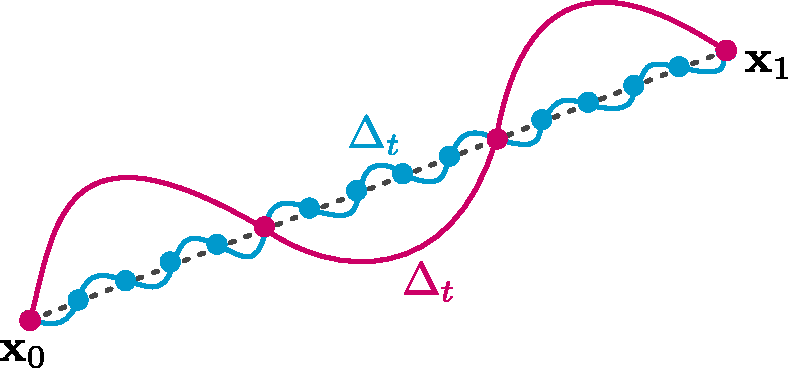
\includegraphics[width = 0.9\textwidth]{images/bounded_joint_path.pdf}
    
    $-$Desired Cartesian path.
    
    \textcolor{uma_pink}{$-$Bounded deviation path with few knots.}
    
    \textcolor{uma_blue_light}{$-$Bounded deviation path with many knots.}
    \end{minipage}%
    \hspace{0.5cm}
    \begin{minipage}{.45\linewidth}
    \textcolor{uma_pink}{\textbf{Low number of knots:}}
        \begin{itemize}
            \item Low computation.
            \item High $\Delta_t$.
            \item High error.
        \end{itemize}
    \textcolor{uma_blue_light}{\textbf{High number of knots:}}
    \begin{itemize}
        \item High computation.
        \item Low $\Delta_t$.
        \item Low error.
    \end{itemize}
    \end{minipage}
    \end{center}

    \framebreak

    \textbf{\textcolor{uma_blue_dark}{Recursive pre-planning method}}

    First, define the maximum position and orientation errors:
    $
    \delta_p^{\textsf{max}} = |p_j(t)-p_{j-1}(t-1)|, \, \delta_r^{\textsf{max}} = |\varphi|
    $
    \begin{enumerate}
        \item Calculate $\mathbf{q}_1$ and $\mathbf{q}_2$ (Inverse Kinematics).
        \item Compute the intermediate joint configuration $\mathbf{q}_i = \mathbf{q}_2-\frac{1}{2}\Delta\mathbf{q}_1$.
        \item Compute the intermediate Cartesian configuration $\mathbf{x}_i = \textsf{Forward Kinematics}(\mathbf{q}_i)$.
        \item Compute the bounded errors $\delta_p$ and $\delta_r$.
        \item Check the bounded errors $\delta_p \leq \delta_p^{\textsf{max}} $ and $\delta_r \leq \delta_r^{\textsf{max}}$.
        \item If the conditions are not satisfied, repeat steps 2 to 5 for the new segments created.
    \end{enumerate}

    Higher errors usually appear at the beginning and end of the trajectories (due to high velocity changes).
    


\end{frame}

\section{Cartesian Interpolation}
\subsection{Homogeneous Matrix Interpolation}
\begin{frame}[allowframebreaks]
\frametitle{Homogeneous Matrix Interpolation}

~\cite{paul1979manipulator}

\end{frame}

\subsection{Interpolation of the Position}
\begin{frame}[allowframebreaks]
\frametitle{Interpolation of the Position}


\end{frame}

\subsection{Interpolation of the Orientation}
\begin{frame}[allowframebreaks]
\frametitle{Interpolation of the Orientation}


\end{frame}


\subsection{Smooth Cartesian Trajectory Planning}
\begin{frame}[allowframebreaks]
\frametitle{Smooth Cartesian Trajectory Planning}


Nowadays, we keep studying this~\cite{tagliavini2023smooth}.

\end{frame}


\section{Optimal Trajectory Planning}
\begin{frame}[allowframebreaks]
\frametitle{Optimal Trajectory Planning}

~\cite{vukobratovic1982method}

\end{frame}


\begin{frame}[allowframebreaks]
\frametitle{Dynamic Scaling of Trajectories}

~\cite{hollerbach1983dynamic}

\end{frame}




\begin{frame}[allowframebreaks]
\frametitle{Bibliography}
\printbibliography
\end{frame}

\end{document}